\subsection{Player \& Ball Detection}
\label{subsec:objectDetectionDesign}
The detection of players and the ball plays a key role in the system. This is performed by using a \textit{YOLOv8-X} Object Detection Model~\cite{yolov8_ultralytics}. The \textit{X} variant of \textit{YOLOv8} is the extra-large version and boast of the highest accuracy was used as it contained the biggest dataset and outperformed other versions. The model was trained via Roboflow on the previously mentioned labelled augmented data, which included bounding boxes for the \texttt{ball}, \texttt{player}, \texttt{goalkeeper}, and \texttt{referee} classes. 

For the training of the model, hyper-parameters needed to be decided. This was done by experimentation which talked about in Section 4. The hyper-parameters and their values are given below:
\begin{itemize}
    \item \textbf{Epochs:} Epochs represent the number of iterations the model goes through whole data for training. A large number of epochs can be computationally expensive and incline towards over-fitting whereas a small value for the number of epochs can cause the model to not learn enough from the data and in turn not generate the results required. A final epoch count of \textbf{50} was opted for.
    \item \textbf{Learning Rate:} The learning rate decides how much the weights in the model should be updated by after each batch. If the learning rate opted for is too large, the weights can overshoot and cause the model to become unstable. On the other hand, a smaller learning rate will take time for training and even might end up fixating at a local minima.
    The final learning rate opted for was \textbf{0.01}.
    \item \textbf{Batch Size:} Batch size represents the number of training samples the model processes before updating its weights. A low batch size causes quick training however can be very noisy. On the other hand, if a batch size chosen is relatively large, the model will learn at a very slow rate and will also require expensive computational resources. Therefore, a batch size of \textbf{8} was used to strike a balance between the model's stability and maximise the \textit{GPU} available.
\end{itemize}

Post the detection of the players and the ball, class-agnostic \textit{Non-Max Suppression (NMS)} is applied to filter out the redundant detections. The final bounding boxes are then wrapped using \texttt{supervision.Detections} objects for further analysis.

A sample of player and ball detection can be seen in Figure~\ref{fig:playerDetection}.

\begin{figure}[H]
    \centering
    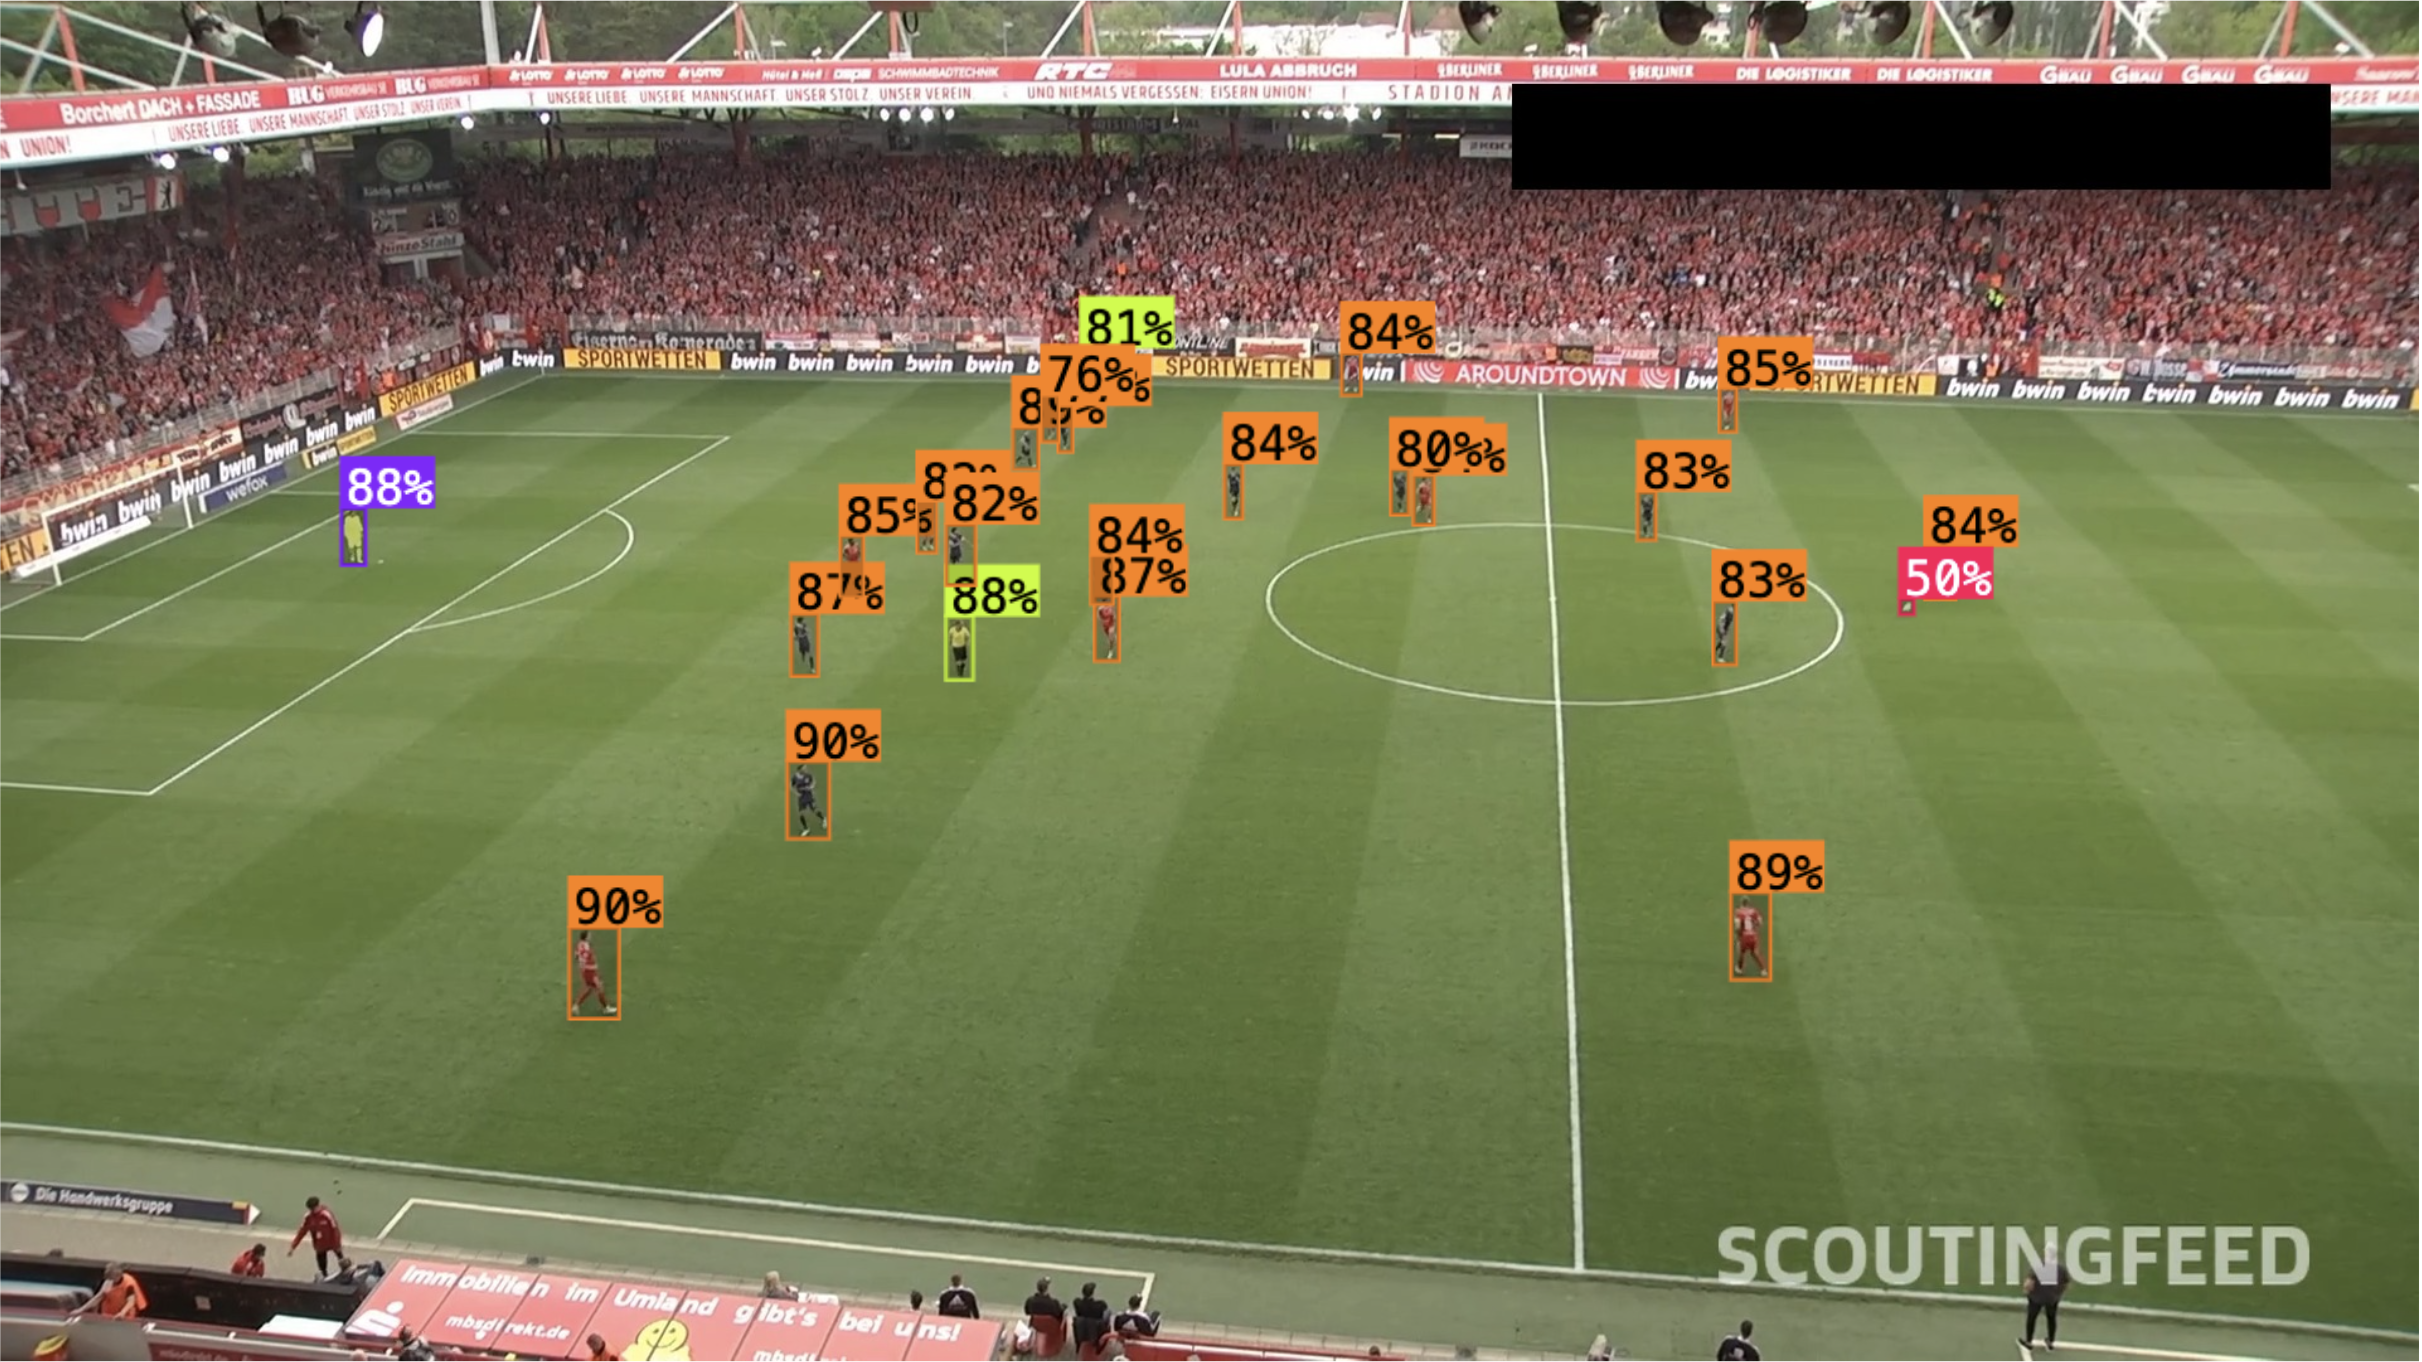
\includegraphics[width=0.7\textwidth]{images/playerDetectionSample.png}
    \caption{Sample Object Detection.}
    \label{fig:playerDetection}
\end{figure}

\subsection{Pitch Keypoint Detection}
\label{subsec:pitchDetectionDesign}

A dedicated \textit{YOLOv8-X} Key-point Detection Model, trained on the labelled pitch data, was employed for the detection of structural field landmarks~\cite{yolov8_ultralytics}. As shown in Figure~\ref{fig:keyPoints}, these include 32 key-points around the pitch, such as the four corners, centre circle extremities, and penalty box vertices. The model outputs 2D coordinates with associated confidence scores for each identified feature.

The training of the model required the selection of hyper-parameters which are talked about as follows:
\begin{enumerate}
    \item \textbf{Epochs:} As stated in Section~\ref{subsec:objectDetectionDesign}, epochs are a key factor in the final model's output. For the pitch detection model, a epoch number of 50 was chosen.
    \item \textbf{Batch Size:} As mentioned previously in Section~\ref{subsec:objectDetectionDesign}, the correct batch size has to be used to strike a balance between speed and stability. Therefore, a batch size of \textbf{16} was opted.
\end{enumerate}


After inference, a confidence threshold is applied to filter out all the low-certainty predictions. This ensures that only the geometrically meaningful and visually reliable key-points are retained. The resulting coordinates are stored as \texttt{supervision.KeyPoints} objects. These objects are used to establish a mapping between a \textit{Bird's Eye View Representation} and their corresponding real-world locations on the pitch which will be talked about later in the report.

\begin{figure}[H]
    \centering
    \includegraphics[width=0.7\textwidth]{images/pitchDetectionSample.png}
    \caption{Sample Pitch Key-Points Detection.}
    \label{fig:pitchDetection}
\end{figure}

Figure~\ref{fig:pitchDetection} shows a sample of the detection of the key-points using the \textit{YOLOv8} Model.

% When a minimum of four high-confidence key-points are available, a homography matrix is computed to project the player and ball positions from the camera frame to a standardized top-down pitch representation, i.e. Bird's Eye View. This transformation is critical for spatial analytics and will be talked about in greater detail in later sections.


